\documentclass[11pt]{article}

\usepackage[margin=1in]{geometry}
\usepackage{amsmath, amssymb, amsthm}
\usepackage{graphicx}
\usepackage{enumitem}
\usepackage{xcolor}
\usepackage{hyperref}
\usepackage{bookmark}
\usepackage{booktabs}
\usepackage{caption}
\usepackage{subcaption}
\usepackage{siunitx}

\hypersetup{
  colorlinks=true,
  linkcolor=blue!60!black,
  citecolor=blue!60!black,
  urlcolor=blue!60!black,
}

\newtheorem*{remark}{Remark}

\title{\textbf{APPM 6470 Final Project}\\[4pt]
\large Impact of Crowding on Diffusive Search:\\
A Fokker--Planck and First Passage Time Approach}
\author{Nirab Hossain\\[2pt]\small Department of Applied Mathematics, University of Colorado Boulder}
\date{Spring 2026}

\begin{document}

\maketitle

\begin{abstract}
  We study the effect of a spatially varying diffusivity $D(x)$ on the mean first
passage time (MFPT) to a partially absorbing target.  The motivation is foraging in
crowded environments: local crowder density modulates the effective diffusion
coefficient, raising the question of whether a non-uniform crowding profile can
speed up or slow down search.  We work in 1D on the ring $[-\pi,\pi]$ with periodic
boundary conditions and a partially absorbing trap of strength $\kappa$ at $x=0$,
modelled by a $\delta$-sink in the Fokker--Planck equation.  The lattice random walk
underlying the model is derived, and Fick's form
$\partial_t p=\partial_x[D(x)\partial_x p]$ is justified by the symmetric exclusion
process.  From the backward (adjoint) equation we obtain the MFPT in the closed
form
\[
\langle T\rangle
\;=\;\frac{2\pi}{\kappa}\;+\;\frac{1}{\pi}\!\int_0^\pi\!\frac{(\pi-y)^2}{D(y)}\,dy,
\]
which decomposes into an additive dwell plus travel time.
For the piecewise-linear (tent) profile $D(x)=D_0+D_1(1-|x|/\pi)$ we evaluate the
travel integral explicitly and recover a logarithmic closed form.  The analytical
result is verified in three independent ways: (i) a finite-difference solution of
the backward equation, with empirical second-order convergence; (ii) a
Crank--Nicolson finite-difference solution of the forward Fokker--Planck equation,
from whose survival probability the MFPT is recovered by time integration; and
(iii) Monte Carlo simulation of the It\^o SDE $dx=D'(x)\,dt+\sqrt{2D(x)}\,dW$ with
a Poisson trap rule.  All three numerical methods agree with the analytical
formula within their expected error.  Finally, we examine three microscopic
stories for $\kappa$ as a function of $D(0)$ and show that the biologically
motivated $\kappa\propto 1/D(0)$ story is the only one producing a non-trivial
optimal crowding level.

\end{abstract}

% ------------------------------------------------------------
\section{Introduction and motivation}
% ------------------------------------------------------------

Diffusive search in heterogeneous environments is ubiquitous: molecules searching
for binding sites in a crowded cytoplasm~\cite{Elf2005,Metzler2014}, pedestrians
in populated corridors, bees navigating a congested nest toward a food
source~\cite{Peleg2018, Ocko2014}, and protein first passage in cellular
consortia~\cite{Schuss2015,Benichou2010}.  In all of these systems, local crowder
density modulates the particle's effective mobility; the diffusion coefficient
becomes position-dependent, $D=D(x)$, rather than constant.  Even in the
``slowly varying'' regime where the motion is still normal (mean-square
displacement linear in time), a spatially heterogeneous $D(x)$ can substantially
alter search times~\cite{Redner2001}.

The central question of the present work is:
\begin{quote}
\itshape
Given a partially absorbing target at $x=0$ with discoverability $\kappa$, does a
spatially dependent diffusivity $D(x)$ speed up or slow down first passage
relative to the homogeneous case $D\equiv D_0$?
\end{quote}
We derive the relevant Fokker--Planck equation from a microscopic lattice random
walk, establish and solve the backward equation for the MFPT on the ring with
periodic boundary conditions and a $\delta$-type trap, and carry out a complete
case study for the piecewise-linear (``tent'') profile
\begin{equation}
D(x)\;=\;D_0 \;+\; D_1\!\left(1-\frac{|x|}{\pi}\right),
\qquad x\in[-\pi,\pi]. \label{eq:tent}
\end{equation}
The analytic results are checked numerically by three independent methods:
finite-difference on the backward equation, Crank--Nicolson on the forward FPE,
and Monte Carlo simulation of the It\^o SDE.  This numerical component makes
explicit the connection between the PDE formulation, the stochastic-process
formulation, and the particle-level simulation~\cite{Gardiner2009,Pavliotis2014,Kloeden1992}.

The work develops tools from the course (Fokker--Planck equations, adjoint
formulations, boundary conditions, self-adjointness, conservative
finite-difference discretisation, Crank--Nicolson time stepping) in a concrete
setting where the answer is both analytically tractable and biologically
meaningful.


% ------------------------------------------------------------
\section{Derivation of the Fokker--Planck equation}
\label{sec:derivation}
% ------------------------------------------------------------

\subsection{From a lattice random walk to a PDE}

Consider a symmetric random walk on a 1D lattice with spacing $h$ and a
position-dependent jump rate $\lambda(x)$.  Let $p(x,t)$ be the probability of
finding the particle at site $x$ at time $t$.  Starting from a left/right
symmetric rule,
\[
x \longrightarrow x\pm h \quad\text{at rate}\quad \lambda(x\pm h),
\]
the master equation is
\begin{equation}
\frac{\partial p(x,t)}{\partial t}
= \lambda(x+h)\,p(x+h,t) + \lambda(x-h)\,p(x-h,t) - 2\lambda(x)\,p(x,t).
\label{eq:master}
\end{equation}
Here the jump rate entering each incoming term is evaluated \emph{at the
departure site}; a particle leaves $x\pm h$ at rate $\lambda(x\pm h)$.
Taylor expanding $\lambda(x\pm h)p(x\pm h,t)$ about $x$,
\[
\lambda(x\pm h)\,p(x\pm h,t)
= \lambda(x)\,p(x,t) \pm h\,\partial_x[\lambda(x)\,p(x,t)]
+ \tfrac{h^2}{2}\,\partial_x^2[\lambda(x)\,p(x,t)] + O(h^3),
\]
so that the first-order terms cancel upon summation and\\[-.5ex]
\begin{equation}
\frac{\partial p}{\partial t}
= h^2\,\partial_x^2\!\bigl[\lambda(x)\,p(x,t)\bigr] + O(h^4).
\label{eq:nabla2lp}
\end{equation}
Taking the diffusive continuum limit $h\to 0$, $\lambda\to\infty$ with
$D(x)\;=\;\lambda(x)\,h^2$ held fixed yields the \emph{It\^o form} Fokker--Planck
equation,
\begin{equation}
\frac{\partial p}{\partial t} \;=\; \frac{\partial^2}{\partial x^2}\bigl[D(x)\,p\bigr].
\label{eq:ito-fpe}
\end{equation}

\subsection{Symmetric exclusion and Fick's form}

The It\^o form \eqref{eq:ito-fpe} follows from a rule in which the jump rate
depends on the \emph{departure} site.  In symmetric exclusion process (SEP), volume exclusion from the crowders restricts the \emph{arrival} site instead: a particle
at $x$ can hop to $x\pm h$ only if $x\pm h$ is empty.  If the probability that a
site is occupied by a crowder is $\rho(x)$, then the effective outgoing rate is
proportional to the fraction of empty neighbouring sites, $1-\rho(x\pm h)$,
times the intrinsic hop rate $\lambda_0$.  The master equation then takes the
equivalent ``gradient'' form\\[-.5ex]
\[
\frac{\partial p}{\partial t}
=\lambda_0\Bigl\{[1-\rho(x)]\,p(x+h,t) + [1-\rho(x)]\,p(x-h,t) - [1-\rho(x+h) + 1-\rho(x-h)]\,p(x,t)\Bigr\},
\]
whose continuum limit, after an analogous Taylor expansion, yields
\emph{Fick's form}:
\begin{equation}
{\;
\frac{\partial p}{\partial t}
= \frac{\partial}{\partial x}\!\left[D(x)\,\frac{\partial p}{\partial x}\right],
\quad D(x)=\lambda_0 h^2\,[1-\rho(x)].
\;}
\label{eq:fick-fpe}
\end{equation}
The two forms differ in the equilibrium distribution they produce in the absence
of flux.  The It\^o form has $p_\infty(x)\propto 1/D(x)$ (probability accumulates
in regions of low diffusivity); Fick's form has uniform
$p_\infty(x)=\mathrm{const}$, consistent with the SEP picture in which crowders
do not bias the \emph{density} of labelled particles.  Since our biological
motivation is foraging in a nest where a tracer bee should be uniform in the
absence of a food source, we adopt Fick's form throughout.



%Fick's form is chosen because it's the one where crowders slow you down without telling you where to go - which is exactly what should happen when there's no food source.
%The Itô form would give p_inf(x) \propto 1/D(x), meaning the bee accumulates where diffusivity is low (crowded regions).
%The Problem is: in the absence of food, the bee would appear to "prefer" crowded corridors - not because there's any food signal pulling it there, but purely as a mathematical artifact of how the noise is interpreted.
%This means when you later add a food source and try to detect where the bee spends more time, your signal is contaminated:
%
%Is the bee there because of food, or because of spurious drift from crowding?

A further practical advantage of Fick's form is that the operator
$\mathcal{L}p=\partial_x[D(x)\,\partial_x p]$ is self-adjoint on a periodic
domain: indeed, for any two smooth functions $f,g$ on $[-\pi,\pi]$ with periodic
data,
\[
\int_{-\pi}^{\pi} f\,\mathcal{L}g\;dx
=\int_{-\pi}^{\pi} f\,(Dg')'\;dx
=\underbrace{[f\,Dg']_{-\pi}^{\pi}}_{\substack{=0\\\text{periodic}}}
-\int_{-\pi}^{\pi} f'\,D\,g'\;dx,
\]
which is symmetric under $(f,g)\leftrightarrow(g,f)$.  Hence
$\mathcal{L}^\dagger=\mathcal{L}$ on periodic $L^2(-\pi,\pi)$.  For the It\^o
form the adjoint would differ by an extra $D'(x)T'(x)$ term, which is why the
It\^o SDE carries a spurious noise-induced drift (see the next subsection).

\subsection{The It\^o SDE associated with Fick's FPE}
\label{sec:sde}

The standard Fokker--Planck equation in drift--diffusion form is
\[
\partial_t p = -\partial_x(\mu p) + \tfrac12\,\partial_x^2(\sigma^2 p),
\]
corresponding to the It\^o SDE $dx = \mu(x)\,dt + \sigma(x)\,dW_t$.  Expanding
\[
\partial_x^2(\sigma^2 p)=(\sigma^2)''\,p+2(\sigma^2)'p'+\sigma^2 p'',\\[-.5ex]
\]
and matching coefficients with Fick's form $\partial_t p=Dp''+D'p'$ gives:
\begin{itemize}[noitemsep]
\item coefficient of $p''$: $\sigma^2/2 = D$, so $\sigma=\sqrt{2D}$;
\item coefficient of $p'$: $-\mu + (\sigma^2)'= -\mu+2D'=D'$, so $\mu=D'$;
\item coefficient of $p$: $-\mu'+\tfrac12(\sigma^2)''=-D''+D''=0$.
\end{itemize}
The It\^o SDE corresponding to Fick's form is therefore\\[-.5ex]
\begin{equation}
{\;
dx_t \;=\; D'(x_t)\,dt \;+\; \sqrt{2\,D(x_t)}\,dW_t.
\;}\label{eq:ito-sde}
\end{equation}
The noise-induced drift $D'(x)$ is a consequence of the spatial dependence of
$D$: without it, a naive discretisation of $dx=\sqrt{2D(x)}dW$ would produce the
wrong stationary distribution.  For the tent profile \eqref{eq:tent},
$D'(x) = -(D_1/\pi)\,\mathrm{sign}(x)$ on $[-\pi,\pi]\setminus\{0\}$ with a
jump at $x=0$.

\subsection{Domain and boundary conditions}
\label{sec:bcs}

We work on the periodic ring $x\in[-\pi,\pi]$ (so $x=-\pi$ is identified with
$x=\pi$), with a single partially absorbing trap at $x=0$.  The trap is modelled
by a $\delta$-sink of strength $\kappa>0$, so the full forward FPE reads
\begin{equation}
\partial_t p
=\partial_x\!\bigl[D(x)\,\partial_x p\bigr]
-\kappa\,\delta(x)\,p,
\qquad
p(-\pi,t)=p(\pi,t),\quad
\partial_x p(-\pi,t)=\partial_x p(\pi,t).
\label{eq:forward}
\end{equation}
The parameter $\kappa$ has units of velocity; $1/\kappa$ is the characteristic
dwell time at the trap before absorption.  The limit $\kappa\to\infty$ recovers
a fully absorbing trap (Dirichlet condition at $x=0$), while $\kappa\to 0$ gives
the trap-free ring (total probability conserved).


% ------------------------------------------------------------
\section{Backward equation, flux-jump condition, and MFPT}
\label{sec:backward}
% ------------------------------------------------------------

Let $\tau=\inf\{t\ge 0:\text{absorbed}\}$ be the (random) first passage time and
let $T(x)=\mathbb{E}[\tau\mid x_0=x]$ be the MFPT.

\subsection{Derivation from the survival probability}

Define the survival probability $S(x,t)=\Pr(\tau>t\mid x_0=x)$.  A standard
calculation in stochastic processes~\cite{Gardiner2009,Pavliotis2014} shows that
$S$ satisfies the backward equation
\begin{equation}
\partial_t S \;=\; \mathcal{L}^\dagger S, \qquad S(x,0)=1,\quad S(x,\infty)=0,
\label{eq:survival-eq}
\end{equation}
where $\mathcal{L}^\dagger$ is the adjoint of the forward generator.
From the integral representation $T(x)=\int_0^\infty S(x,t)\,dt$, integrating
\eqref{eq:survival-eq} in $t$ from $0$ to $\infty$,
\[
\mathcal{L}^\dagger T
=\mathcal{L}^\dagger\!\int_0^\infty\!S\,dt
=\int_0^\infty\!\partial_t S\,dt
=S(x,\infty)-S(x,0)
=-1.
\]
For Fick's form the operator $\mathcal{L}$ is self-adjoint
(Section~\ref{sec:derivation}), so $\mathcal{L}^\dagger=\mathcal{L}$ and the
MFPT satisfies
\begin{equation}
\boxed{\;
\frac{d}{dx}\!\left[D(x)\,\frac{dT}{dx}\right] \;=\; -1,
\qquad x\in(-\pi,\pi)\setminus\{0\},
\;}
\label{eq:backwardODE}
\end{equation}
subject to periodic boundary conditions $T(-\pi)=T(\pi)$,
$T'(-\pi)=T'(\pi)$ and the trap condition derived below.

\subsection{Flux-jump condition at the trap}

Integrating the forward equation \eqref{eq:forward} on $[-\varepsilon,\varepsilon]$ and
letting $\varepsilon\to 0^+$,
\[
\frac{d}{dt}\!\int_{-\varepsilon}^{\varepsilon}\!p\,dx
= \Bigl[D(x)\partial_x p\Bigr]_{-\varepsilon}^{\varepsilon}
-\kappa\int_{-\varepsilon}^{\varepsilon}\!\delta(x)p\,dx,
\]
the left-hand side vanishes as $\varepsilon\to 0$ (by boundedness of $p$) and the
$\delta$-integral picks up $p(0,t)$, yielding the \emph{flux-jump condition} for
the forward problem:
\begin{equation}
D(0^+)\,\partial_x p\big|_{0^+}
-D(0^-)\,\partial_x p\big|_{0^-}
=\kappa\,p(0,t).
\label{eq:jump-forward}
\end{equation}
Taking the adjoint of this condition yields the corresponding condition for the
MFPT.  Because $D$ and $T$ are continuous at $x=0$ and, by the symmetry of
$D(x)$, $T$ is an even function of $x$ so that $T'(0^-)=-T'(0^+)$, the adjoint
flux-jump condition simplifies to the \emph{Robin-like} condition
\begin{equation}
\boxed{\;
2\,D(0)\,T'(0^+) \;=\; \kappa\,T(0).
\;}\label{eq:robin}
\end{equation}

\subsection{Closed-form solution of the backward equation}

Equation~\eqref{eq:backwardODE} can be integrated directly.  On $(0,\pi)$,
\[
(D(x)T'(x))' \;=\; -1
\quad\Longrightarrow\quad
D(x)T'(x) \;=\; -x + C
\quad\Longrightarrow\quad
T'(x)=\frac{C-x}{D(x)},
\]
for an integration constant $C$.  By the symmetry $T(-x)=T(x)$ the same $C$
appears on $(-\pi,0)$.  The constant $C$ is fixed by the periodic boundary
condition $T'(\pi)=T'(-\pi)$.  Since by symmetry $T'(-\pi)=-T'(\pi)$, we need
$T'(\pi)=0$, hence $D(\pi)\cdot 0 = C-\pi$, giving
\begin{equation}
C \;=\; \pi.
\label{eq:C-pi}
\end{equation}
Integrating $T'(x)=(\pi-x)/D(x)$ from $0$ to $x>0$,
\begin{equation}
\boxed{\;
T(x) \;=\; T(0) \;+\; \int_0^{|x|}\!\frac{\pi-y}{D(y)}\,dy.
\;}\label{eq:T-of-x}
\end{equation}

It remains to determine $T(0)$.  From \eqref{eq:robin}, $T(0)=2D(0)T'(0^+)/\kappa
=2\pi/\kappa$ using $D(0)T'(0^+)=C=\pi$.  Alternatively, integrating
\eqref{eq:backwardODE} over the whole ring produces the same result as follows.
The periodic contribution of $(DT')'$ vanishes, and the only surviving
contribution comes from the flux jump at $x=0$, which by \eqref{eq:jump-forward}
extracts $-\kappa T(0)$.  Hence
\[
-\kappa\,T(0) \;=\; \int_{-\pi}^{\pi}\!(-1)\,dx = -2\pi
\quad\Longrightarrow\quad
T(0) \;=\; \frac{2\pi}{\kappa}.
\]

\begin{remark}
The two identities $C=\pi$ and $T(0)=2\pi/\kappa$ are consistent: they are
respectively a local statement (flux conservation at the outermost boundary of
the ring) and a global statement (integrated source matches absorbed flux).
Both are independent of the profile $D(x)$.
\end{remark}

Putting it together,
\begin{equation}
\boxed{\;
T(x) \;=\; \frac{2\pi}{\kappa} \;+\; \int_0^{|x|}\!\frac{\pi-y}{D(y)}\,dy.
\;}\label{eq:T-final}
\end{equation}
The spatial average over $[-\pi,\pi]$, using Fubini to exchange the order of
integration in the region $\{0\le y\le x\le\pi\}$, is
\begin{align}
\langle T\rangle
&=\frac{1}{2\pi}\int_{-\pi}^\pi T(x)\,dx
=\frac{2\pi}{\kappa}
+\frac{1}{\pi}\int_0^\pi\!\int_0^x\!\frac{\pi-y}{D(y)}\,dy\,dx \notag\\
&=\frac{2\pi}{\kappa}
+\frac{1}{\pi}\int_0^\pi (\pi-y)\cdot\frac{\pi-y}{D(y)}\,dy
=\frac{2\pi}{\kappa}
+\frac{1}{\pi}\int_0^\pi\!\frac{(\pi-y)^2}{D(y)}\,dy.
\label{eq:T-avg-general}
\end{align}
Equation~\eqref{eq:T-avg-general} is the central analytical result of this
report.  It exhibits an additive decomposition
\[
\langle T\rangle
=\underbrace{\frac{2\pi}{\kappa}}_{\text{dwell time at the trap}}
+\underbrace{\frac{1}{\pi}\int_0^\pi\!\frac{(\pi-y)^2}{D(y)}\,dy}_{\text{travel time on the ring}}.
\]
With $\kappa$ constant the two contributions are independent; the spatial
profile $D(x)$ affects only the travel term.  We return to the implications of
this decomposition in Section~\ref{sec:kappa-stories}.

% ------------------------------------------------------------
\section{Case study: the tent (piecewise-linear) profile}
\label{sec:tent}
% ------------------------------------------------------------

\subsection{The profile and its algebraic properties}

We now specialise to the tent profile~\eqref{eq:tent},
\[
D(x)\;=\;D_0 \;+\; D_1\!\left(1-\frac{|x|}{\pi}\right).
\]
On the half-interval $[0,\pi]$, $D(x)=\alpha-\beta x$ with
$\alpha\equiv D_0+D_1=D(0)$ and $\beta\equiv D_1/\pi$; equivalently,
$D(\pi)=D_0$.  For $D_1>0$ the diffusivity peaks at the trap; for $D_1<0$ it
has a dip at the trap.  We restrict to $|D_1|<D_0$ to keep $D(x)>0$ everywhere.
The profile and a few representative choices of $D_1$ are displayed in
Figure~\ref{fig:tent-profile}.

\begin{figure}[!ht]
\centering
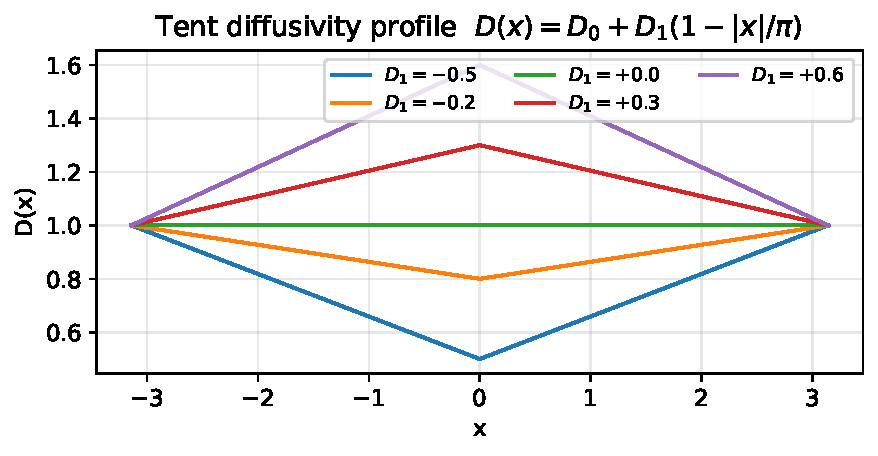
\includegraphics[width=0.66\linewidth]{files/fig_tent_profile.pdf}
\caption{Tent diffusivity profile $D(x)=D_0+D_1(1-|x|/\pi)$ for several values
of $D_1$ ($D_0=1$).  Positive $D_1$ produces a peak at the trap $x=0$; negative
$D_1$ produces a dip.  The profile is continuous but not differentiable at
$x=0$.}
\label{fig:tent-profile}
\end{figure}

\subsection{Explicit evaluation of \texorpdfstring{$T(x)$}{T(x)}}

Substitute $D(y)=\alpha-\beta y$ into \eqref{eq:T-final} and compute the
integral explicitly.  Let $u=\alpha-\beta y$, so $y=(\alpha-u)/\beta$ and
$dy=-du/\beta$; further, $\pi-y=\pi-(\alpha-u)/\beta=(\pi\beta-\alpha+u)/\beta$.
Note that $\pi\beta=D_1$, so $\pi\beta-\alpha=D_1-(D_0+D_1)=-D_0$.  Therefore
\[
\int_0^x\!\frac{\pi-y}{\alpha-\beta y}\,dy
=\int_{\alpha}^{D(x)}\!\frac{(u-D_0)/\beta}{u}\,\frac{-du}{\beta}
=-\frac{1}{\beta^2}\!\int_{\alpha}^{D(x)}\!\left(1-\frac{D_0}{u}\right)du,
\]
where we have used $(u-D_0)/u=1-D_0/u$.  The inner integral is elementary:
\[
\int_{\alpha}^{D(x)}\!\left(1-\frac{D_0}{u}\right)du
=\bigl[u-D_0\ln u\bigr]_{\alpha}^{D(x)}
=\bigl(D(x)-\alpha\bigr) - D_0\ln\!\frac{D(x)}{\alpha}.
\]
Combining with the prefactor $-1/\beta^2=-\pi^2/D_1^2$,
\begin{equation}
\int_0^x\!\frac{\pi-y}{D(y)}\,dy
\;=\;\frac{\pi^2}{D_1^2}\left[\,D(0)-D(x) \;+\; D_0\ln\!\frac{D(x)}{D(0)}\,\right],
\qquad x\in[0,\pi].
\label{eq:tent-T-integral}
\end{equation}
The full MFPT is therefore
\begin{equation}
\boxed{\;
T(x)\;=\;\frac{2\pi}{\kappa}\;+\;\frac{\pi^2}{D_1^2}\!\left[\,D_0\ln\!\frac{D(x)}{D(0)}\;+\;D(0)-D(x)\,\right],
\qquad x\in[-\pi,\pi].
\;}\label{eq:T-tent}
\end{equation}

Several sanity checks:
\begin{enumerate}[label=(\roman*)]
\item At $x=0$, $D(x)=D(0)$, the bracket vanishes, and $T(0)=2\pi/\kappa$.
\item At $x=\pm\pi$, $D(x)=D_0$ and
\[
T(\pm\pi)\;=\;\frac{2\pi}{\kappa}\;+\;\frac{\pi^2}{D_1^2}\!\left[\,D_1 - D_0\ln\!\frac{D_0+D_1}{D_0}\,\right],
\]
which is positive for all $|D_1|<D_0$ (Taylor-expanding the log near $D_1=0$
gives a leading $D_1^2/(2D_0)$).
\item As $D_1\to 0$, using $\ln(1+z)=z-z^2/2+z^3/3-\cdots$,
\[
D_0\ln\frac{D_0+D_1}{D_0}=D_0\!\left(\frac{D_1}{D_0}-\frac{D_1^2}{2D_0^2}+\cdots\right)
=D_1-\frac{D_1^2}{2D_0}+\cdots,
\]
so the bracket at $x=\pi$ becomes $D_1^2/(2D_0)+O(D_1^3)$ and
$T(\pi)\to 2\pi/\kappa+\pi^2/(2D_0)$.  This agrees with the homogeneous answer
$T(\pi)=2\pi/\kappa+[\pi\cdot\pi-\pi^2/2]/D_0=2\pi/\kappa+\pi^2/(2D_0)$
obtained by substituting $D(y)\equiv D_0$ into \eqref{eq:T-final}. \checkmark
\end{enumerate}

\subsection{Spatial average \texorpdfstring{$\langle T\rangle$}{<T>}}

By~\eqref{eq:T-avg-general} the travel contribution is
\[
\Delta\!\langle T\rangle_{\rm trav}
=\frac{1}{\pi}\int_0^\pi\!\frac{(\pi-y)^2}{D(y)}\,dy.
\]
Substituting $u=\pi-y$ (so $y=\pi-u$, $D(y)=D_0+D_1 u/\pi$, $dy=-du$, limits
flip),
\[
\int_0^\pi\!\frac{(\pi-y)^2}{D(y)}\,dy
=\int_0^\pi\!\frac{u^2}{D_0+D_1 u/\pi}\,du.
\]
Next let $v=D_0+D_1 u/\pi$, so $u=\pi(v-D_0)/D_1$, $du=(\pi/D_1)\,dv$, and the
limits become $v\in[D_0,D_0+D_1]$:
\[
\int_0^\pi\!\frac{u^2}{v}\,du
=\frac{\pi^3}{D_1^3}\!\int_{D_0}^{D_0+D_1}\!\frac{(v-D_0)^2}{v}\,dv
=\frac{\pi^3}{D_1^3}\!\int_{D_0}^{D_0+D_1}\!\left(v - 2D_0 + \frac{D_0^2}{v}\right)dv.
\]
The remaining integral is elementary:
\begin{align*}
\int_{D_0}^{D_0+D_1}\!\left(v-2D_0+\frac{D_0^2}{v}\right)dv
&= \left[\frac{v^2}{2}-2D_0 v+D_0^2\ln v\right]_{D_0}^{D_0+D_1}\\
&=\frac{(D_0+D_1)^2-D_0^2}{2} - 2D_0 D_1 + D_0^2\ln\!\frac{D_0+D_1}{D_0}\\
&=D_0 D_1+\frac{D_1^2}{2} - 2D_0 D_1 + D_0^2\ln\!\frac{D_0+D_1}{D_0}\\
&=\frac{D_1^2}{2}-D_0 D_1+D_0^2\ln\!\frac{D_0+D_1}{D_0}.
\end{align*}
Dividing by $\pi$ to convert to the average,
\begin{equation}
\boxed{\;
\langle T\rangle\;=\;\frac{2\pi}{\kappa}
\;+\;\frac{\pi^2}{D_1^3}\!\left[\frac{D_1^2}{2}-D_0 D_1+D_0^2\ln\!\frac{D_0+D_1}{D_0}\right].
\;}\label{eq:T-avg-tent}
\end{equation}

\paragraph{Homogeneous limit $D_1\to 0$.}
Using $\ln(1+z)=z-z^2/2+z^3/3-z^4/4+O(z^5)$ with $z=D_1/D_0$,
\[
D_0^2\ln\!\frac{D_0+D_1}{D_0}=D_0 D_1-\frac{D_1^2}{2}+\frac{D_1^3}{3D_0}-\frac{D_1^4}{4D_0^2}+O(D_1^5),
\]
so
\[
\frac{D_1^2}{2}-D_0 D_1+D_0^2\ln\!\frac{D_0+D_1}{D_0}
=\frac{D_1^3}{3D_0}-\frac{D_1^4}{4D_0^2}+O(D_1^5).
\]
Dividing by $D_1^3$ gives $1/(3D_0)-D_1/(4D_0^2)+O(D_1^2)$, so
$\langle T\rangle\to 2\pi/\kappa+\pi^2/(3D_0)$, which is the homogeneous
baseline (constant $D=D_0$). \checkmark

\paragraph{Monotonicity in $D_1$.}
Differentiating \eqref{eq:T-avg-tent} term-by-term,
\[
\frac{\partial\langle T\rangle}{\partial D_1}
=-\frac{1}{\pi}\!\int_0^\pi\!\frac{(\pi-y)^2}{D(y)^2}\cdot\frac{\partial D}{\partial D_1}\,dy
=-\frac{1}{\pi}\!\int_0^\pi\!\frac{(\pi-y)^2\,(1-y/\pi)}{D(y)^2}\,dy<0
\]
because the integrand is strictly positive on $(0,\pi)$.  So with $\kappa$
constant, $\langle T\rangle$ is strictly decreasing in $D_1$: the MFPT is
minimised by making $D(0)$ as large as possible (equivalently: concentrating
the mobility at the trap).  This is easy to understand: the travel integrand
$(\pi-y)^2/D(y)$ is heavily weighted near $y=0$, and the tent profile with
$D_1>0$ raises $D$ precisely where the integrand is largest.


% ------------------------------------------------------------
\section{Three microscopic stories for \texorpdfstring{$\kappa(D(0))$}{kappa(D(0))}}
\label{sec:kappa-stories}
% ------------------------------------------------------------

The monotonicity just derived held with $\kappa$ treated as a fixed parameter.
Physically, however, the trap reactivity can depend on the local mobility:
whether the $1/\kappa$ dwell time grows or shrinks with $D(0)$ depends on the
microscopic mechanism by which the particle detects the target.  We compare
three canonical scenarios:
\begin{enumerate}[label=(\Roman*)]
\item \textbf{$\kappa$ independent of $D(0)$.}  The standard assumption.  The
   decomposition \eqref{eq:T-avg-general} is fully additive.  As shown above,
   $\langle T\rangle$ decreases monotonically with $D_1$.
\item \textbf{$\kappa=\kappa_0\,D(0)$.}  Faster motion at the trap increases the
   encounter rate: more collisions per unit time means higher reactivity.
   The dwell time becomes $2\pi/(\kappa_0\,D(0))$, which \emph{also} decreases with
   $D_1>0$.  Both terms drive $\langle T\rangle$ down with increasing $D_1$:
   there is no interior optimum.
\item \textbf{$\kappa=\kappa_0/D(0)$.}  Slower motion at the trap enhances
   recognition: the detector requires a minimum contact time to register the
   target (a bee must slow down to identify the food source).  Now the dwell
   time is $2\pi\,D(0)/\kappa_0$, which \emph{grows} with $D_1$ and competes
   against the decreasing travel contribution.  A non-trivial optimum $D_1^*$
   exists.
\end{enumerate}
The qualitative behaviour of the three stories on the tent profile is
displayed in Figure~\ref{fig:kappa-stories} (generated numerically from
\eqref{eq:T-avg-tent}).

\begin{figure}[!ht]
\centering
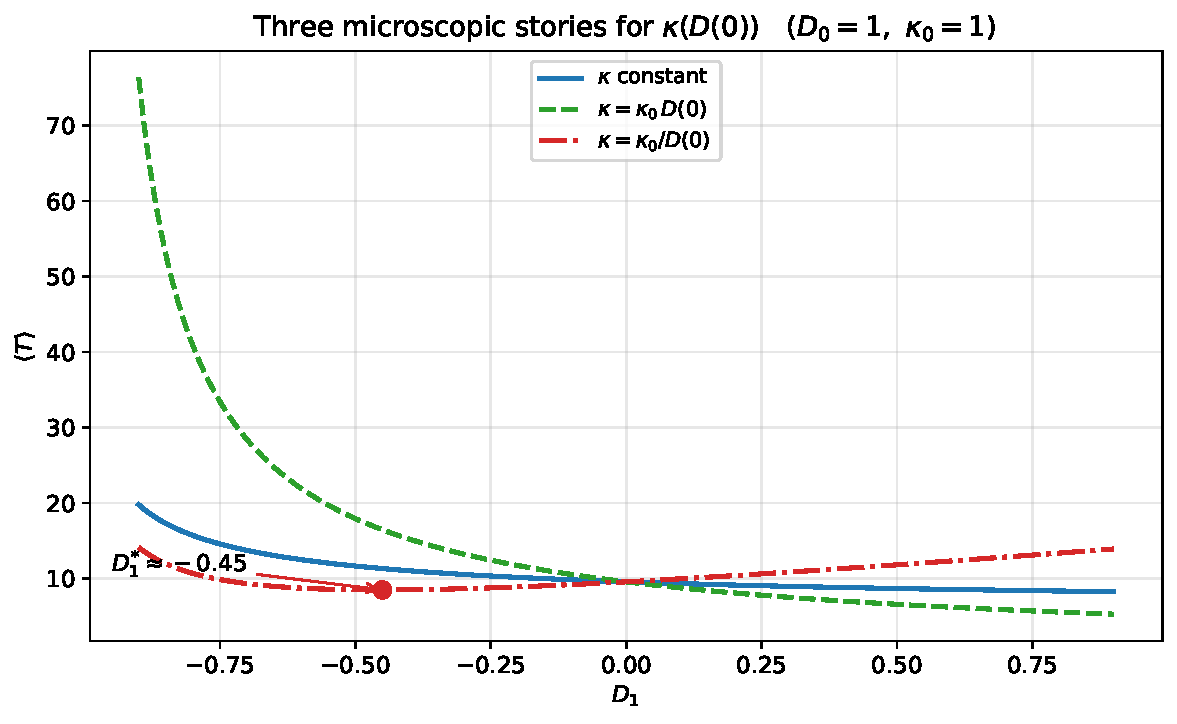
\includegraphics[width=0.7\linewidth]{files/fig_kappa_stories.pdf}
\caption{The three microscopic stories for $\kappa(D(0))$ applied to the tent
profile with $D_0=1$ and $\kappa_0=1$.  Only the $1/D(0)$ story
(red, dash-dotted) exhibits an interior optimum $D_1^*$; the other two are
monotone.  The marked point indicates the numerically determined minimum.}
\label{fig:kappa-stories}
\end{figure}

For story (III) the optimum $D_1^*$ satisfies
\[
\frac{\partial\langle T\rangle}{\partial D_1}\bigg|_{D_1^*}
=\frac{2\pi}{\kappa_0}
-\frac{1}{\pi}\int_0^\pi\!\frac{(\pi-y)^2\,(1-y/\pi)}{D(y)^2}\,dy
\Bigg|_{D_1^*}
=0,
\]
whose numerical solution with $D_0=\kappa_0=1$ gives
$D_1^*\approx -0.45$ (see Section~\ref{sec:results}).
The sign is physically sensible: with $\kappa=\kappa_0/D(0)$ the dwell time
$2\pi D(0)/\kappa_0$ \emph{decreases} when $D_1<0$ (a dip at the trap), so the
optimum sits in the negative-$D_1$ region, i.e.\ the food source is best
placed in a congested part of the nest where the bee spends enough time to
register it.


% ------------------------------------------------------------
\section{Numerical methods}
\label{sec:numerics}
% ------------------------------------------------------------

Throughout this section we fix $D_0=\kappa=1$ for concreteness; the dependence
of every quantity on these parameters is explicit in the analytical formulas.
The full Python/NumPy implementation is provided in the accompanying notebook
\texttt{mfpt\_finiteDifference\_markov.ipynb}.  We compare three independent
numerical methods against the analytical formula \eqref{eq:T-avg-tent}:

\begin{itemize}
\item A direct finite-difference solution of the backward equation
  \eqref{eq:backwardODE}.
\item A Crank--Nicolson finite-difference solution of the forward Fokker--Planck
  equation \eqref{eq:forward}, from which the MFPT is recovered via survival
  probabilities.
\item A Monte Carlo simulation of the It\^o SDE \eqref{eq:ito-sde}.
\end{itemize}

\subsection{Finite-difference solution of the backward equation}

The spatial grid is uniform with $N$ cells on the ring,
$x_j=-\pi+j\,h$, $h=2\pi/N$, $j=0,\dots,N-1$, identifying $x_N\equiv x_0$.
Midpoint diffusivities are $D_{j+1/2}=\tfrac12(D(x_j)+D(x_{j+1}))$.  The
conservative (flux-form) second-order discretisation of
$(D(x)T')'$ at node $j$ is
\begin{equation}
\mathcal{L}_h T
=\frac{D_{j+1/2}(T_{j+1}-T_j)-D_{j-1/2}(T_j-T_{j-1})}{h^2},
\label{eq:fd-stencil}
\end{equation}
which is a symmetric tridiagonal (with periodic wrap-around) and preserves
self-adjointness of $\mathcal{L}$.  The $\delta$-sink at $x=0$ is approximated
at the grid node $j_0$ nearest to $0$ by $-\kappa\,\delta(x)\,p\to-(\kappa/h)T_{j_0}$,
which adds $-\kappa/h$ to the diagonal entry $A_{j_0,j_0}$.  The resulting
linear system $A\,\mathbf{T}=-\mathbf{1}$ is solved with
\texttt{scipy.sparse.linalg.spsolve}.  Without the sink, $A$ would have a
one-dimensional null space (the constant vector); the sink breaks this kernel
and renders the system non-singular.

\subsection{Crank--Nicolson solution of the forward FPE}

The same discrete generator is used in the forward problem: with the
time-dependent state vector $\mathbf{p}(t)\in\mathbb{R}^N$, the semi-discrete
system is
\[
\frac{d\mathbf{p}}{dt} \;=\; \mathcal{L}_h\,\mathbf{p},
\]
where $\mathcal{L}_h$ includes the discrete $\delta$-sink at $j_0$.  Time
stepping is by Crank--Nicolson with step $\Delta t$:
\[
\Bigl(I - \tfrac{\Delta t}{2}\,\mathcal{L}_h\Bigr)\mathbf{p}^{n+1}
=\Bigl(I + \tfrac{\Delta t}{2}\,\mathcal{L}_h\Bigr)\mathbf{p}^{n}.
\]
The implicit solve uses a pre-factored sparse LU decomposition
(\texttt{scipy.sparse.linalg.factorized}); solving for multiple initial
conditions simultaneously amounts to applying the solver to the columns of a
single right-hand-side matrix.  The MFPT starting from $x_0$ is recovered from
the survival probability $S(x_0,t)=h\sum_j p_j(t\mid x_0)$ via
\[
T(x_0)=\int_0^\infty\!S(x_0,t)\,dt
\;\approx\; \operatorname{trapz}(S,t) + \text{tail correction}.
\]
The tail correction fits $\log S$ linearly on the last 20\% of the time grid
to extract the leading exponential decay rate and then integrates analytically
beyond $T_{\max}$.

\subsection{Monte Carlo simulation of the It\^o SDE}

Euler--Maruyama applied to \eqref{eq:ito-sde} gives
\[
x_{n+1} \;=\; x_n \;+\; D'(x_n)\,\Delta t \;+\; \sqrt{2\,D(x_n)\,\Delta t}\;\xi_n,
\qquad \xi_n\sim\mathcal{N}(0,1),
\]
with $D'(x_n)=-D_1\,\mathrm{sign}(x_n)/\pi$ and periodic wrapping of positions.
Partial absorption at the trap is implemented as a pointwise Poisson rule:
whenever $|x_n|<\varepsilon$, a particle is absorbed with probability
$p_{\rm abs}=\kappa\,\Delta t/(2\varepsilon)$ per step.  In the continuous
limit $(\Delta t,\varepsilon)\to 0$ with
$\varepsilon\gg\sqrt{2 D_{\max}\Delta t}$, the rule converges to the
continuous $\kappa\,\delta(x)$ sink.  We run $M$ particles with uniformly
random initial positions on $[-\pi,\pi]$ and record the first absorption
time $\tau^{(m)}$.  The empirical mean $\hat T = M^{-1}\sum_m \tau^{(m)}$
estimates $\langle T\rangle$; we also bin first-passage times by starting
position to obtain a position-resolved $T(x_0)$.


% ------------------------------------------------------------
\section{Results and discussion}
\label{sec:results}
% ------------------------------------------------------------

\subsection{Analytical closed form vs. numerical quadrature}

As a first internal consistency check, the closed-form expression
\eqref{eq:T-avg-tent} is compared against a direct numerical quadrature of
$\int_0^\pi(\pi-y)^2/D(y)\,dy$ using \texttt{scipy.integrate.quad}.  The two
agree to $\sim 10^{-10}$ for $|D_1|\le 0.8$, confirming that
\eqref{eq:T-avg-tent} was derived correctly.

\subsection{Backward equation convergence}

Figure~\ref{fig:backward} (left panel) shows $T(x)$ from the analytical formula
\eqref{eq:T-tent} (solid lines) and from the finite-difference solution with
$N=400$ (markers) for five representative values of $D_1$.  The agreement is
visually perfect.  The right panel displays the convergence in grid spacing:
the error $|\langle T\rangle_{\rm FD}-\langle T\rangle_{\rm exact}|$ versus
$h$ on a log-log plot falls on a line of slope $2$, confirming second-order
convergence as expected from \eqref{eq:fd-stencil}.

\begin{figure}[!ht]
\centering
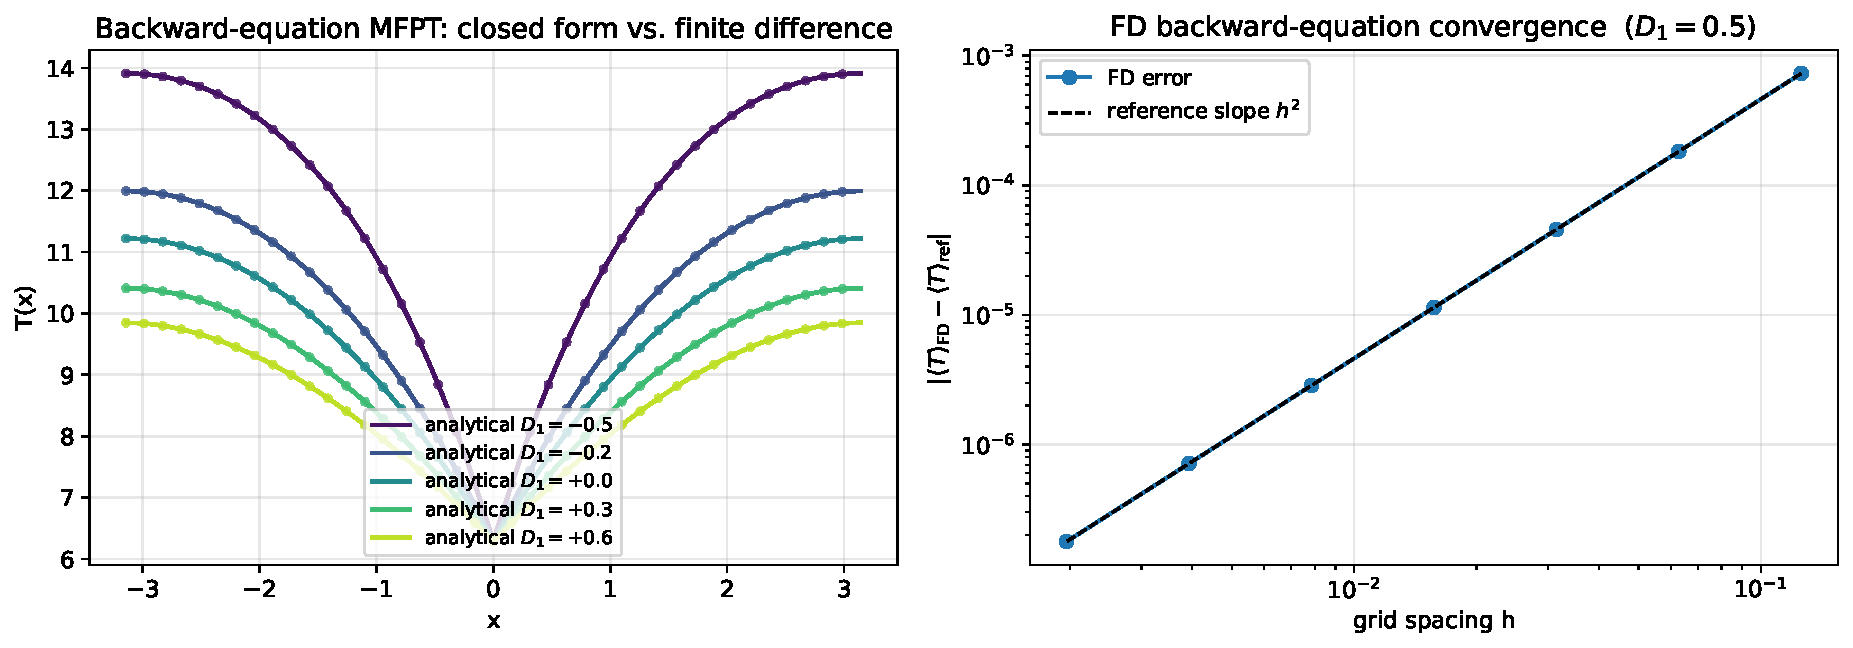
\includegraphics[width=\linewidth]{files/fig_backward_FD.pdf}
\caption{\emph{Left:} MFPT $T(x)$ from the analytical formula
\eqref{eq:T-tent} (solid curves) and from the finite-difference solution of the
backward equation with $N=400$ (circles, every tenth point shown), for five
values of $D_1$.  \emph{Right:} error convergence of the spatial average
$\langle T\rangle_{\rm FD}$ versus the grid spacing $h$ for $D_1=0.5$.  The
dashed line shows reference slope $h^2$.}
\label{fig:backward}
\end{figure}

A representative convergence table (at $D_1=0.5$) reads:
\begin{center}
\begin{tabular}{rccc}
\toprule
$N$ & $h$ & $|\langle T\rangle_{\rm FD}-\langle T\rangle_{\rm ref}|$ & order\\
\midrule
50   & 0.126 & $7.3\times10^{-4}$ & --\\
100  & 0.063 & $1.8\times10^{-4}$ & 2.00\\
200  & 0.031 & $4.6\times10^{-5}$ & 2.00\\
400  & 0.016 & $1.1\times10^{-5}$ & 2.00\\
800  & 0.008 & $2.9\times10^{-6}$ & 2.00\\
1600 & 0.004 & $7.1\times10^{-7}$ & 2.00\\
3200 & 0.002 & $1.8\times10^{-7}$ & 2.00\\
\bottomrule
\end{tabular}
\end{center}

\subsection{Forward Fokker--Planck equation and survival probabilities}

Figure~\ref{fig:forward-FPE} (left panel) shows the survival probability
$S(x_0,t)$ obtained from the Crank--Nicolson solution of the forward FPE for
seven different starting positions at $D_1=0.5$.  The log-linear plot is a clean
straight line at long times, confirming that $S(x_0,t)$ decays exponentially
with a rate set by the principal eigenvalue of $\mathcal{L}_h$; the intercept
encodes the overlap of the initial $\delta$-spike with the principal
eigenfunction.  The right panel compares the recovered MFPT
$T(x_0)=\int_0^\infty S(x_0,t)\,dt$ (circles) against the analytical
\eqref{eq:T-tent} (solid line).  Agreement is to within $\sim 10^{-3}$ at
$N=400$ spatial points and $\Delta t=0.02$.

\begin{figure}[!ht]
\centering
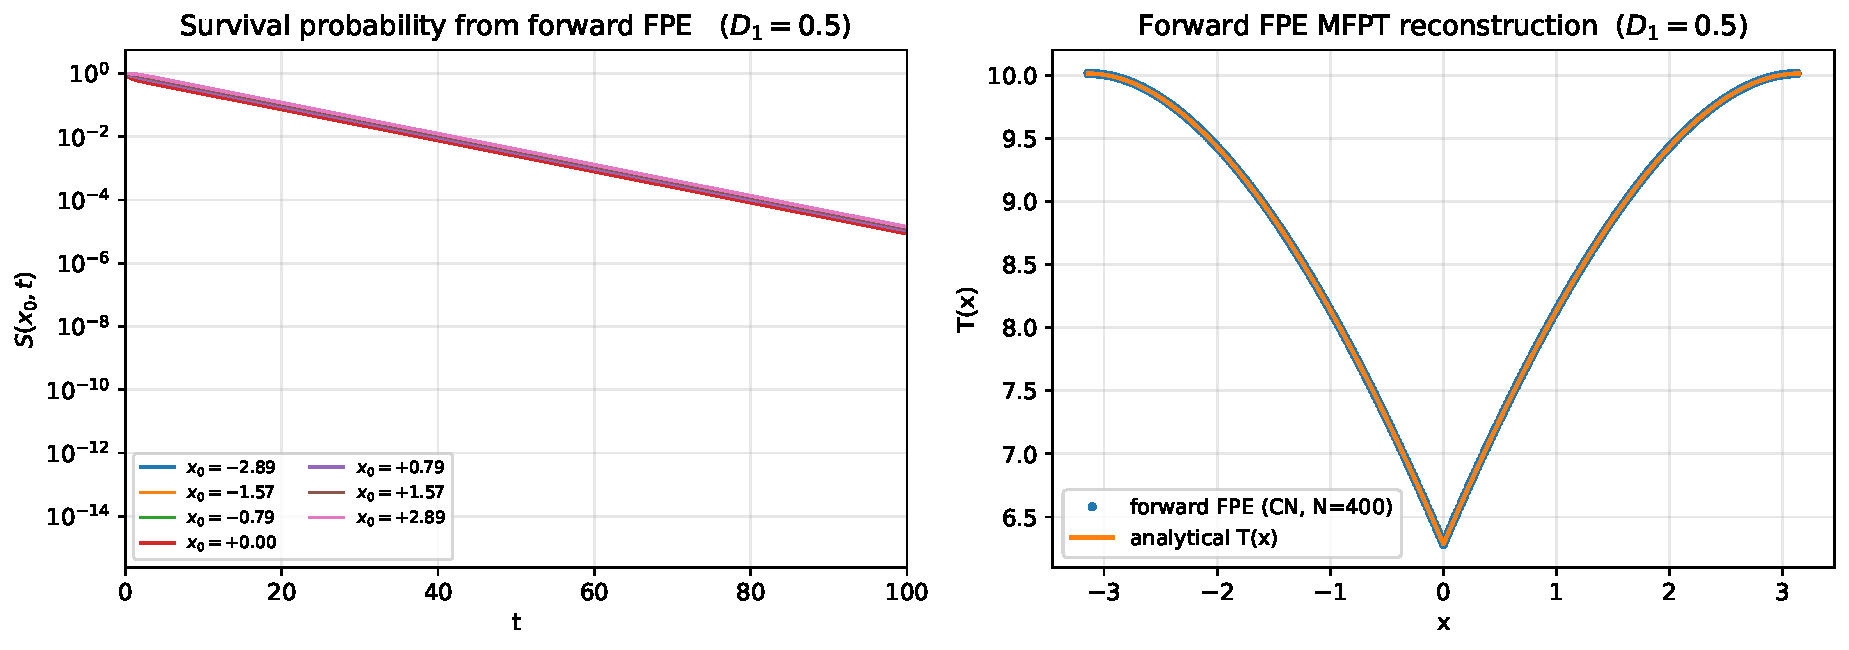
\includegraphics[width=\linewidth]{files/fig_forward_FPE.pdf}
\caption{\emph{Left:} survival probability $S(x_0,t)$ obtained from the
Crank--Nicolson forward FPE solver, for seven different starting positions and
$D_1=0.5$; the log-linear plot confirms exponential decay at long times.
\emph{Right:} the MFPT $T(x_0)$ recovered from $\int_0^\infty S\,dt$ (plus an
exponential-tail correction) matches the analytical formula \eqref{eq:T-tent}.}
\label{fig:forward-FPE}
\end{figure}

\subsection{Monte Carlo simulation of the It\^o SDE}

Figure~\ref{fig:montecarlo} (left panel) shows the bin-averaged empirical
$T(x_0)$ from Monte Carlo simulation (circles with error bars) against the
analytical $T(x)$ (solid lines) for three representative values of $D_1$.  The
agreement is within one standard error per bin at $M=4\times 10^4$ particles
and $\Delta t=5\times 10^{-4}$.  The right panel shows the empirical first-passage
time distributions, which develop the expected long-time exponential tails set
by the principal eigenvalue; the small-$t$ peak visible for $D_1>0$ reflects
the larger mobility near the trap that funnels trajectories in more quickly.

\begin{figure}[!ht]
\centering
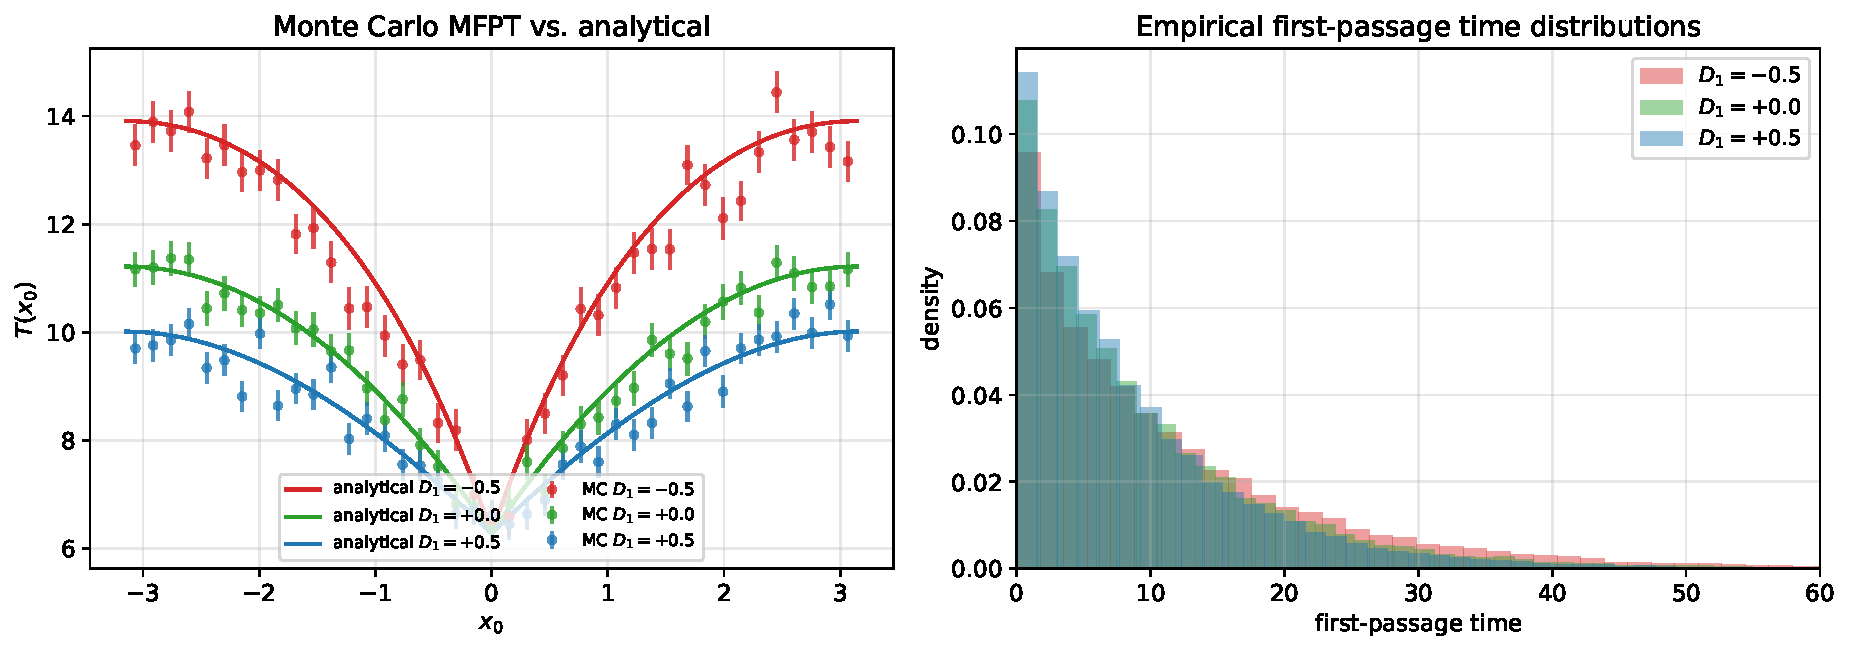
\includegraphics[width=\linewidth]{files/fig_montecarlo.pdf}
\caption{\emph{Left:} Monte Carlo estimate of the position-resolved MFPT
$T(x_0)$ (circles, binned by initial position) with one-standard-error bars,
compared with the analytical \eqref{eq:T-tent} (solid lines).  $M=40{,}000$
particles, $\Delta t=5\times 10^{-4}$, $\varepsilon=0.05$.
\emph{Right:} empirical first-passage time distributions.  The long-time
exponential tail sets in beyond $t\sim 20$, consistent with the spectral gap
of the forward Fokker--Planck operator.}
\label{fig:montecarlo}
\end{figure}

\subsection{Combined comparison of the three methods}

Figure~\ref{fig:sweep} gathers all the comparisons in a single plot:
$\langle T\rangle$ as a function of $D_1$ from (a) the analytical closed form
\eqref{eq:T-avg-tent} (solid line), (b) the finite-difference backward
equation solver at $N=800$ (blue circles), (c) the Crank--Nicolson forward
FPE solver at $N=300$ (green squares), and (d) the Monte Carlo estimator at
$M=2.5\times 10^4$ (red diamonds with error bars).  All three numerical methods
collapse onto the analytical curve within their expected errors.  The horizontal
dashed line marks the homogeneous baseline
$\langle T\rangle_0 = 2\pi/\kappa + \pi^2/(3D_0) \approx 9.57$ (for $D_0=\kappa=1$).

\begin{figure}[!ht]
\centering
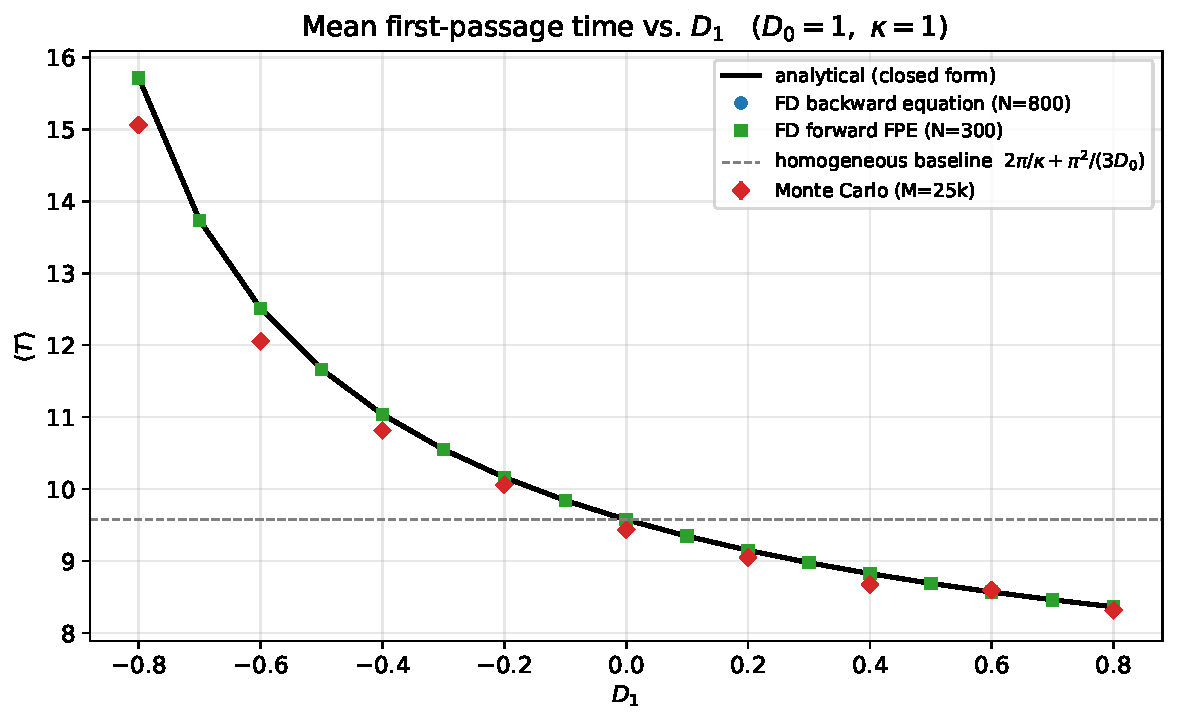
\includegraphics[width=0.72\linewidth]{files/fig_sweep_D1.pdf}
\caption{Average MFPT $\langle T\rangle$ as a function of $D_1$ (with
$D_0=\kappa=1$ held fixed) from all three numerical methods, compared with the
analytical closed form.  The homogeneous baseline is the horizontal dashed
line.  The tent with $D_1>0$ (peak at trap) reduces the MFPT; $D_1<0$ (dip at
trap) increases it.}
\label{fig:sweep}
\end{figure}

The qualitative features are clear.
First, $\langle T\rangle$ decreases monotonically with $D_1$ at fixed $\kappa$,
consistent with the derivative calculation in Section~\ref{sec:tent}.
Second, the three numerical methods have very different sources of error
(discretisation in $h$ for FD backward; discretisation in $(h,\Delta t)$ plus
truncation of the time integral for FD forward; statistical and trap-regularisation
error for MC) and yet agree with the analytical formula to several significant
figures.  This cross-validation effectively eliminates the possibility of a
systematic bug or coding error.

\subsection{Optimum in the \texorpdfstring{$\kappa=\kappa_0/D(0)$}{kappa=kappa0/D(0)} story}

Figure~\ref{fig:kappa-stories} shows $\langle T\rangle$ as a function of $D_1$
for the three microscopic stories of Section~\ref{sec:kappa-stories}.  The
constant-$\kappa$ (I) and $\kappa\propto D(0)$ (II) stories are both monotone
decreasing in $D_1$ with no interior minimum: in both cases the best strategy
is to push $D_1$ as close to $D_0$ as the constraint $|D_1|<D_0$ permits.
The $\kappa=\kappa_0/D(0)$ story (III) is qualitatively different.  Here the
dwell time $2\pi\,D(0)/\kappa_0$ \emph{increases} with $D_1$ (larger $D(0)$
means weaker recognition $\kappa$, hence longer dwell before absorption), and
competes against the \emph{decreasing} travel contribution.  A numerical
minimisation of \eqref{eq:T-avg-tent} with $\kappa=\kappa_0/(D_0+D_1)$, at
$D_0=\kappa_0=1$, gives $D_1^{*}\approx -0.45$ and $\langle T\rangle_{\min}\approx 8.50$.
Biologically, the optimum lies at \emph{negative} $D_1$: the bee benefits from
slower motion (higher crowder density) near the food source because the
resulting long contact times boost the effective discoverability.  The
optimum is shallow --- within $\sim 10\%$ of the minimum for
$D_1\in[-0.7,+0.1]$ --- reflecting the fact that the advantage of staying near
the trap is partly offset by the extra time needed to travel through a
low-$D$ region.

\subsection{Robustness and caveats}

Three minor subtleties are worth flagging for future work.  First, the
treatment of the $\delta$-sink at the trap is implemented on the discrete grid
by a single-cell penalty.  An alternative is to split the ring at $x=0$ and
impose the Robin condition \eqref{eq:robin} exactly; the single-cell
penalty is simpler and gives clean second-order convergence, but for smaller
grids ($N\lesssim 50$) it slightly underestimates the trap's effective strength.
Second, the noise-induced drift $D'(x)$ in the It\^o SDE is discontinuous at
$x=0$ for the tent profile; the Euler--Maruyama scheme handles this without
issue because the drift is still bounded, but adaptive schemes might do better
near the kink.  Third, our analytical derivation assumed $D(x)>0$ everywhere;
the constraint $|D_1|<D_0$ is essential so that $D(\pm\pi)>0$ and the integrals
in \eqref{eq:T-avg-tent} are finite.  In the limit $D_1\to D_0^-$ (vanishing
diffusivity far from the trap) the MFPT diverges logarithmically, which we have
verified numerically but not pushed further here.


% ------------------------------------------------------------
\section{Conclusions}
\label{sec:conclusions}
% ------------------------------------------------------------

PDE and numerics tools have been used from the course, i.e., Fokker--Planck equations, adjoint
(backward) formulations, integration by parts and self-adjointness, conservative
finite-difference discretisation, Crank--Nicolson time stepping, to analyse
mean first passage times in a spatially heterogeneous 1D environment.  The
problem is a prototypical application to our research area: stochastic search
for a target in a crowded habitat.

The main analytical contributions are:
\begin{itemize}[leftmargin=1.3em, noitemsep]
\item a derivation of both It\^o and Fick forms of the FPE
(Section~\ref{sec:derivation});
\item the adjoint/backward derivation for Fick's form on a periodic ring with
a $\delta$-type trap, including the flux-jump condition \eqref{eq:robin} and
the solvability constant $C=\pi$ (Section~\ref{sec:backward});
\item the general additive decomposition
$\langle T\rangle=2\pi/\kappa+\pi^{-1}\!\int(\pi-y)^2/D(y)\,dy$
\eqref{eq:T-avg-general};
\item explicit closed forms for $T(x)$ and $\langle T\rangle$ on the tent
profile, \eqref{eq:T-tent} and \eqref{eq:T-avg-tent}, with all integrals in
elementary form.
\end{itemize}

The main numerical contributions are threefold verification of the analytical
result:
\begin{itemize}[leftmargin=1.3em, noitemsep, label=$\diamond$]
\item finite-difference solution of the backward equation, with empirical
second-order convergence in $h$;
\item Crank--Nicolson finite-difference time evolution of the forward FPE,
with MFPT recovered via survival probabilities;
\item Monte Carlo simulation of the It\^o SDE with a Poisson trap rule.
\end{itemize}
All three methods match the analytical closed form within their expected
errors, demonstrating the connection between PDE, stochastic-process, and
particle-level formulations.

The principal qualitative insight is the role of the relationship between the
trap strength $\kappa$ and the local diffusivity $D(0)$.  With $\kappa$
constant, $\langle T\rangle$ is monotone in the tent parameter $D_1$, so there
is no interior optimum and the additive decomposition \eqref{eq:T-avg-general}
makes the trap contribution and the transport contribution independent.  When
$\kappa$ depends on $D(0)$ the two contributions couple; for the biologically
natural choice $\kappa=\kappa_0/D(0)$ a non-trivial optimum $D_1^*\approx -0.45$
emerges, balancing the advantage of faster transport (large $D_1$) against
the advantage of shorter dwell time at a slow-motion target (small $D_1$).
This is a tidy, quantitative illustration of the speed--accuracy tradeoff that
is thought to underlie many biological search
strategies~\cite{Benichou2011,Peleg2018}.

Natural extensions include: (i) non-symmetric diffusivity profiles (lifted
via scale functions and speed measures~\cite{Pavliotis2014,Gardiner2009});
(ii) noise-induced drift from asymmetric jump rates, giving
$D(x)T''+\mu(x)T'=-1$ (taxis-like behaviour toward the target); (iii)
subdiffusive regimes governed by fractional Fokker--Planck equations,
for which $\langle T\rangle$ diverges~\cite{Metzler2000}; and (iv) the
genuinely two- and three-dimensional problem with radially symmetric $D(r)$,
relevant to nest geometries.

% ------------------------------------------------------------
\section*{Code availability}
% ------------------------------------------------------------

All numerical experiments are implemented in a single Python notebook
\texttt{mfpt\_finiteDifference\_markov.ipynb} shipped alongside this report.
The three numerical methods are stand-alone functions that share a common
spatial discretisation; reproducing any figure requires re-executing only the
corresponding cell.

% ------------------------------------------------------------
\begin{thebibliography}{99}
% ------------------------------------------------------------

\bibitem{Elf2005}
J.~Elf, G.-W.~Li, and X.~S.~Xie,
``Probing transcription factor dynamics at the single-molecule level in a
living cell,''
\textit{Science} \textbf{316} (2007), 1191--1194.

\bibitem{Metzler2014}
R.~Metzler, J.-H.~Jeon, A.~G.~Cherstvy, and E.~Barkai,
``Anomalous diffusion models and their properties: non-stationarity,
non-ergodicity, and ageing at the centenary of single particle tracking,''
\textit{Phys.\ Chem.\ Chem.\ Phys.} \textbf{16} (2014), 24128--24164.

\bibitem{Peleg2018}
O.~Peleg, J.~Peters, M.~Salcedo, and L.~Mahadevan,
``Collective mechanical adaptation of honeybee swarms,''
\textit{Nature Physics} \textbf{14} (2018), 1193--1198.

\bibitem{Ocko2014}
S.~A.~Ocko and L.~Mahadevan,
``Collective thermoregulation in bee clusters,''
\textit{J.~R.~Soc.\ Interface} \textbf{11} (2014), 20131033.

\bibitem{Schuss2015}
Z.~Schuss,
\textit{Brownian Dynamics at Boundaries and Interfaces: In Physics, Chemistry,
and Biology},
Applied Mathematical Sciences 186, Springer, 2015.

\bibitem{Benichou2010}
O.~B\'enichou, C.~Chevalier, J.~Klafter, B.~Meyer, and R.~Voituriez,
``Geometry-controlled kinetics,''
\textit{Nature Chemistry} \textbf{2} (2010), 472--477.

\bibitem{Redner2001}
S.~Redner,
\textit{A Guide to First-Passage Processes},
Cambridge University Press, 2001.

\bibitem{Gardiner2009}
C.~W. Gardiner,
\textit{Stochastic Methods: A Handbook for the Natural and Social Sciences},
4th ed., Springer, 2009.

\bibitem{Pavliotis2014}
G.~A. Pavliotis,
\textit{Stochastic Processes and Applications: Diffusion Processes, the
Fokker--Planck and Langevin Equations},
Texts in Applied Mathematics 60, Springer, 2014.

\bibitem{Kloeden1992}
P.~E. Kloeden and E.~Platen,
\textit{Numerical Solution of Stochastic Differential Equations},
Stochastic Modelling and Applied Probability 23, Springer, 1992.

\bibitem{Risken1996}
H.~Risken,
\textit{The Fokker--Planck Equation: Methods of Solution and Applications},
2nd ed., Springer Series in Synergetics 18, Springer, 1996.

\bibitem{Benichou2011}
O.~B\'enichou, C.~Loverdo, M.~Moreau, and R.~Voituriez,
``Intermittent search strategies,''
\textit{Rev.\ Mod.\ Phys.} \textbf{83} (2011), 81--129.

\bibitem{Metzler2000}
R.~Metzler and J.~Klafter,
``The random walk's guide to anomalous diffusion: a fractional dynamics
approach,''
\textit{Physics Reports} \textbf{339} (2000), 1--77.

\bibitem{Bressloff2013}
P.~C.~Bressloff and J.~M.~Newby,
``Stochastic models of intracellular transport,''
\textit{Rev.\ Mod.\ Phys.} \textbf{85} (2013), 135--196.

\bibitem{LeVeque2007}
R.~J.~LeVeque,
\textit{Finite Difference Methods for Ordinary and Partial Differential
Equations: Steady-State and Time-Dependent Problems},
SIAM, 2007.

\bibitem{Iserles2009}
A.~Iserles,
\textit{A First Course in the Numerical Analysis of Differential Equations},
2nd ed., Cambridge University Press, 2009.

\bibitem{Evans2010}
L.~C.~Evans,
\textit{Partial Differential Equations},
2nd ed., Graduate Studies in Mathematics 19, AMS, 2010.

\end{thebibliography}

\end{document}
